\documentclass[12pt,a4paper]{article}
\usepackage{graphicx}
\usepackage[english,ngerman]{babel}
\usepackage[parfill]{parskip} % to start each parapraph will an empty line before
\usepackage{listings}
\usepackage{hyperref}
\usepackage{float}

\begin{document}
	\begin{titlepage}
		\centering
		
\includegraphics[width=0.8\textwidth]{img/Hska_logo.png}\par\vspace{1cm}
		{\scshape\LARGE Dokumentation\par}
		\vspace{1.5cm}
		{\huge\bfseries Verteilte Systeme Master Labor\par}
		\vspace{2cm}
		{\Large\itshape Pol Zeimet (65834) \\\href{mailto:zepo1012@hs-karlsruhe.de}{zepo1012@hs-karlsruhe.de}\par}
		\vfill
		{\Large\itshape Yannick Stephan (65934) \\\href{mailto:stya1012@hs-karlsruhe.de}{stya1012@hs-karlsruhe.de}\par}
		\vfill
		\large Aufgabe 3
		
		\vfill
		
		% Bottom of the page
		{\large \today\par}
	\end{titlepage}
	\section{Architekturentwurf}
	\label{sec:Architekturentwurf}	
		\begin{figure}[h]
			\centering
			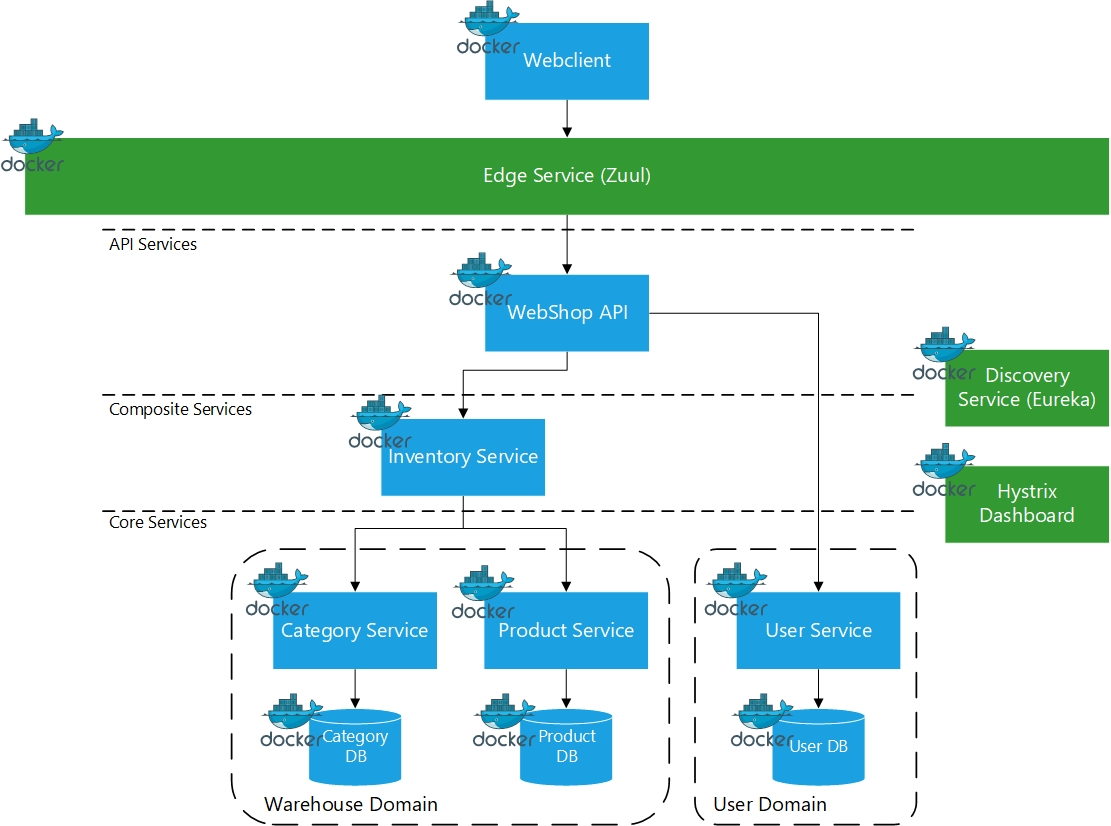
\includegraphics[scale=0.65]{diagrams/architecture_v2.jpg}
			\caption{Implementierte Systemarchitektur}
			\label{fig:microservices-architecture}
		\end{figure}
\end{document}